\section{Results}

	\subsection{Quiz Results}

		\subsubsection{Aggregate Quiz Scores}

			\begin{figure}[h] 
			\centering 
			\begin{minipage}[b]{0.45\linewidth}
			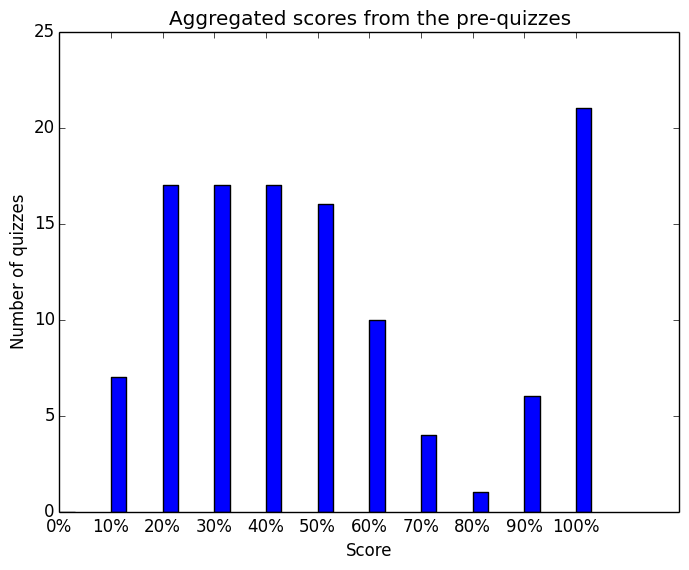
\includegraphics[height=0.33\textheight]{general_pre.png} 
			\caption{The aggregate pre-quiz scores across all games.}
			\end{minipage}
			\quad
			\begin{minipage}[b]{0.45\linewidth}
			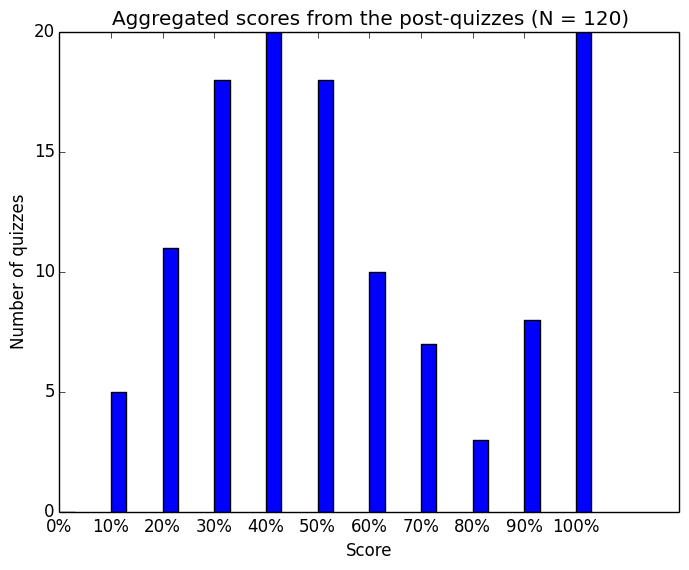
\includegraphics[height=0.33\textheight]{general_post.png} 
			\caption{The aggregate post-quiz scores across all games.}
			\end{minipage}
			\end{figure}

			\begin{figure}[h] 
			\centering 
			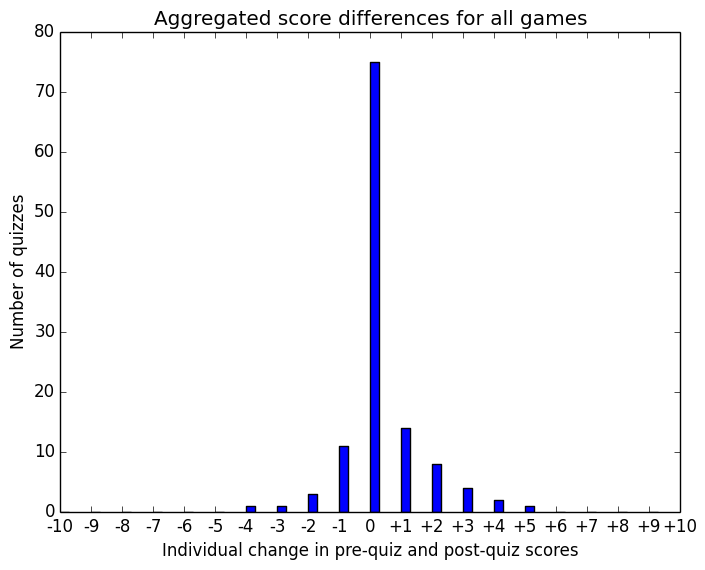
\includegraphics[height=0.33\textheight]{general_results.png} 
			\caption{The aggregate score differences across all games.}
			\end{figure}

	\cleardoublepage

		\subsubsection{Darfur Quiz Scores}

			\begin{figure}[h] 
			\centering 
			\begin{minipage}[b]{0.45\linewidth}
			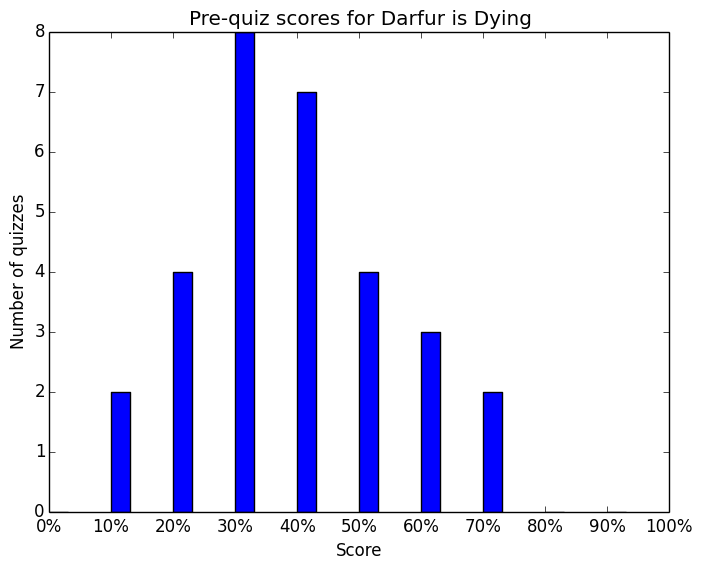
\includegraphics[height=0.33\textheight]{darfur_pre.png} 
			\caption{The pre-quiz scores for Darfur is Dying.}
			\end{minipage}
			\quad
			\begin{minipage}[b]{0.45\linewidth}
			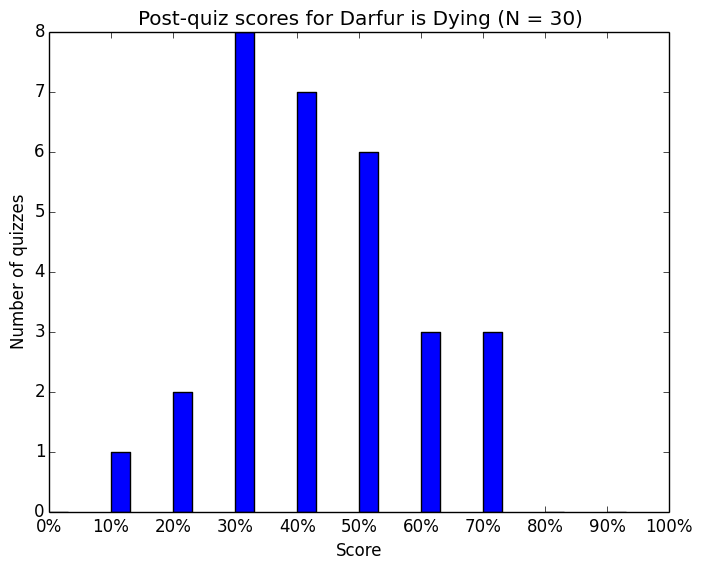
\includegraphics[height=0.33\textheight]{darfur_post.png} 
			\caption{The post-quiz scores for Darfur is Dying.}
			\end{minipage}
			\end{figure}

			\begin{figure}[h] 
			\centering 
			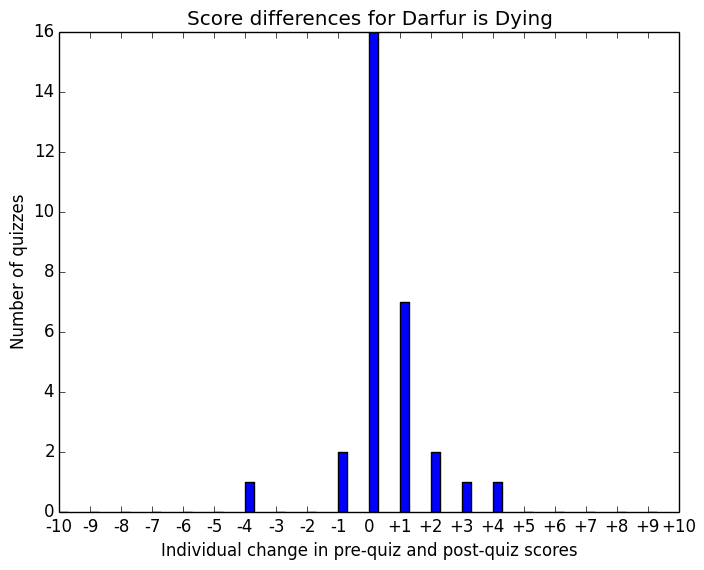
\includegraphics[height=0.33\textheight]{darfur_results.png} 
			\caption{The score differences for Darfur is Dying.}
			\end{figure}


	\cleardoublepage

		\subsubsection{The Oregon Trail Quiz Scores}

			

			\begin{figure}[h] 
			\centering 
			\begin{minipage}[b]{0.45\linewidth}
			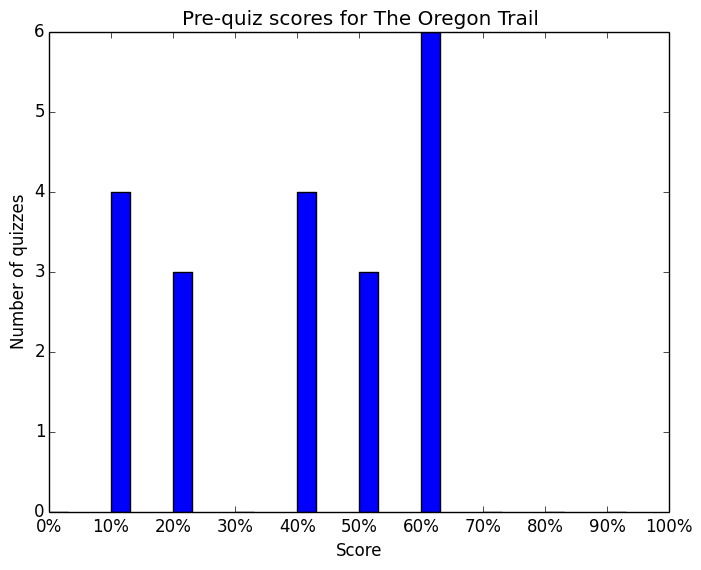
\includegraphics[height=0.33\textheight]{oregon_pre.png} 
			\caption{The pre-quiz scores for The Oregon Trail.}
			\end{minipage}
			\quad
			\begin{minipage}[b]{0.45\linewidth}
			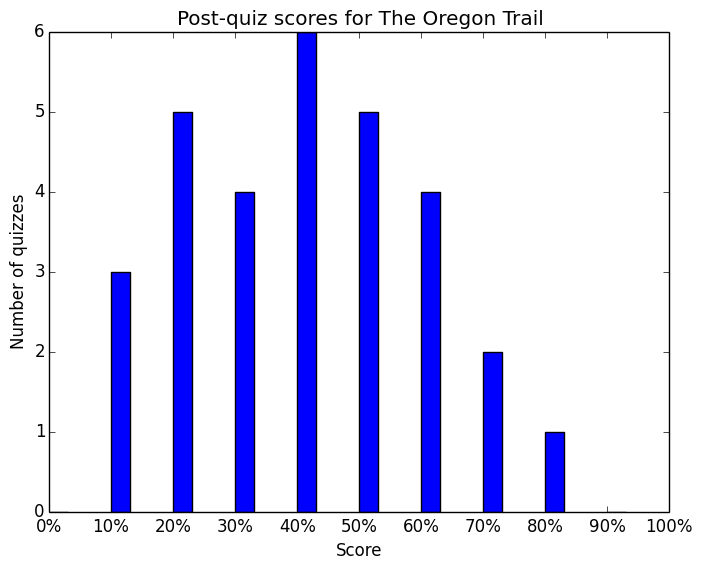
\includegraphics[height=0.33\textheight]{oregon_post.png} 
			\caption{The post-quiz scores for The Oregon Trail.}
			\end{minipage}
			\end{figure}
			
			\begin{figure}[h] 
			\centering 
			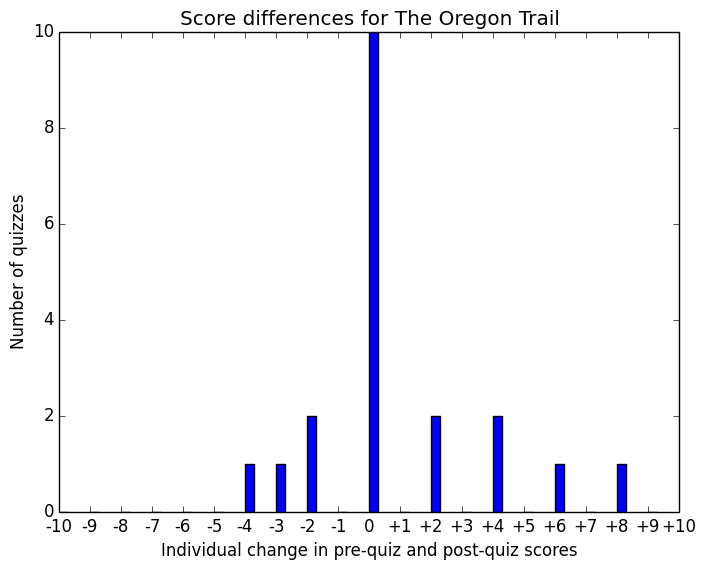
\includegraphics[height=0.33\textheight]{oregon_results.png} 
			\caption{The score differences for The Oregon Trail.}
			\end{figure}

	\cleardoublepage

		\subsubsection{Number Munchers Quiz Scores}

			

			\begin{figure}[h] 
			\centering 
			\begin{minipage}[b]{0.45\linewidth}
			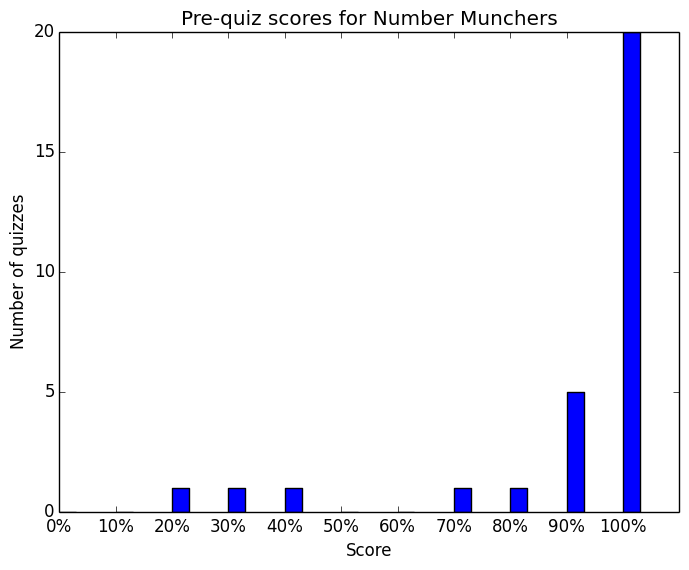
\includegraphics[height=0.33\textheight]{munchers_pre.png} 
			\caption{The pre-quiz scores for Number Munchers.}
			\end{minipage}
			\quad
			\begin{minipage}[b]{0.45\linewidth}
			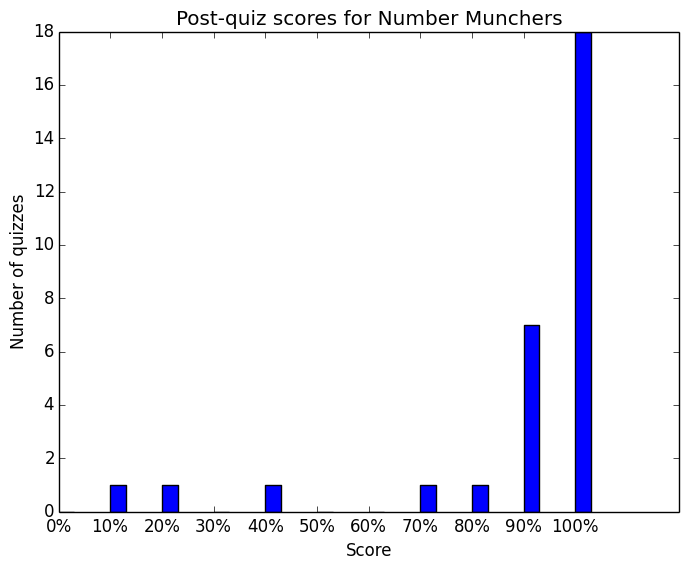
\includegraphics[height=0.33\textheight]{munchers_post.png} 
			\caption{The post-quiz scores for Number Munchers.}
			\end{minipage}
			\end{figure}

			\begin{figure}[h] 
			\centering 
			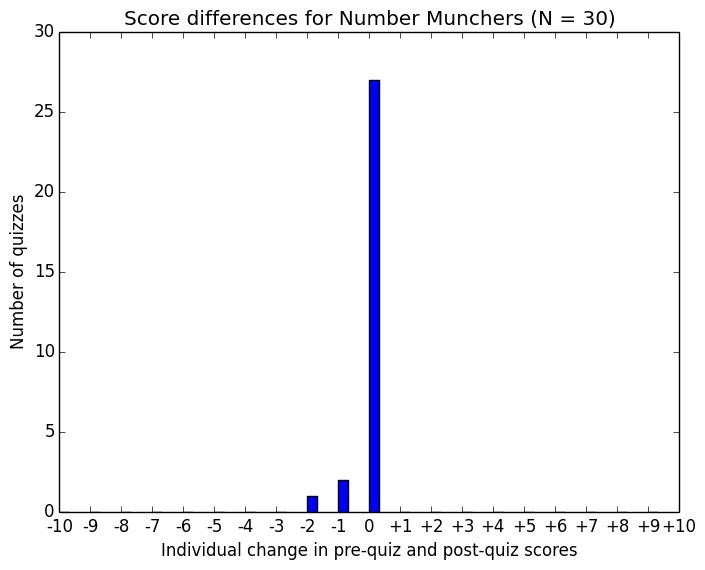
\includegraphics[height=0.33\textheight]{munchers_results.png} 
			\caption{The score differences for Number Munchers.}
			\end{figure}


\cleardoublepage

		\subsubsection{Light Bot Quiz Scores}

			

			\begin{figure}[h] 
			\centering 
			\begin{minipage}[b]{0.45\linewidth}
			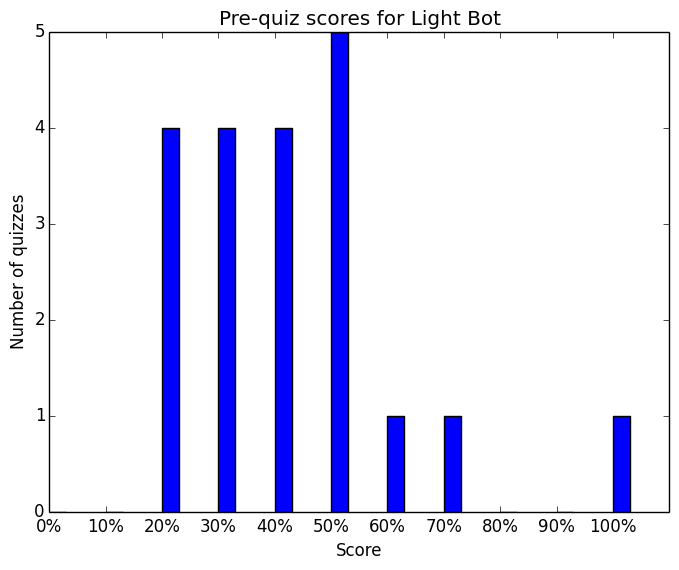
\includegraphics[height=0.33\textheight]{lightbot_pre.png} 
			\caption{The pre-quiz scores for Light Bot.}
			\end{minipage}
			\quad
			\begin{minipage}[b]{0.45\linewidth}
			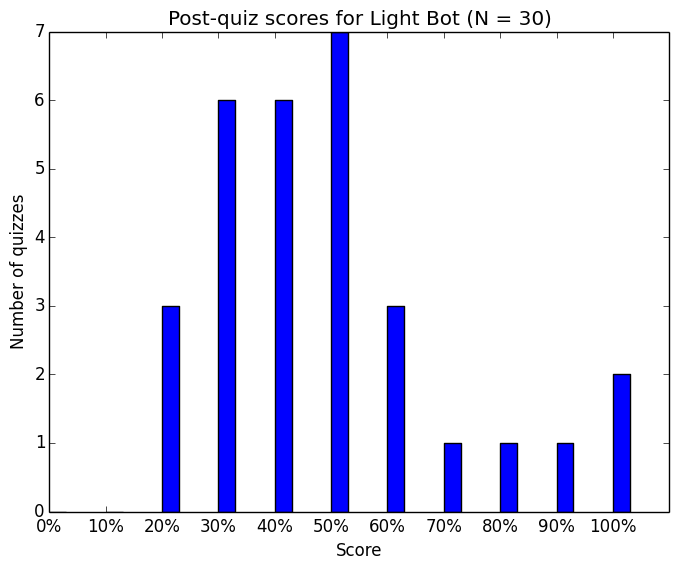
\includegraphics[height=0.33\textheight]{lightbot_post.png} 
			\caption{The post-quiz scores for Light Bot.}
			\end{minipage}
			\end{figure}

			\begin{figure}[h] 
			\centering 
			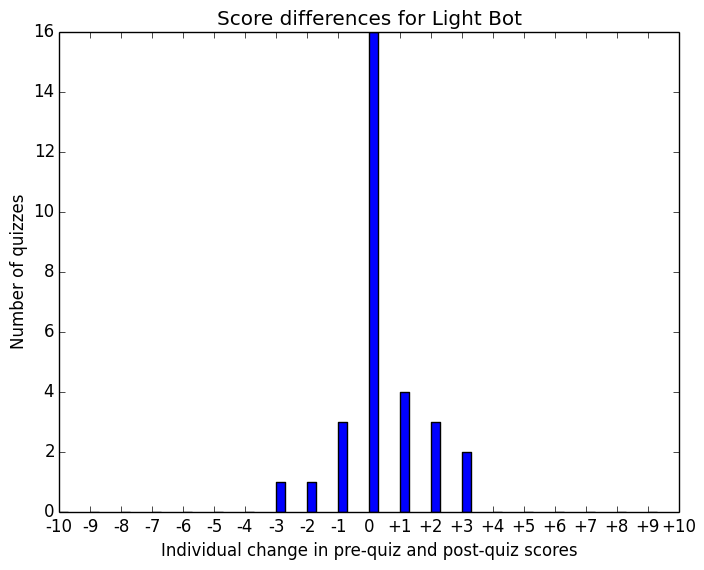
\includegraphics[height=0.33\textheight]{lightbot_results.png} 
			\caption{The score differences for Light Bot.}
			\end{figure}







\cleardoublepage

		\subsection{Rubric Scores}
			This section contains the scoring results for each rubric item. For each rubric item, a bar graph is given for each game. The bar graph contains the scores that the game recieved for that rubric item.

			An alternate visualization of this data, where each game has a bar graph for all of the rubric items, can be found in the next section.

			\begin{figure}[h] 
			\centering 
			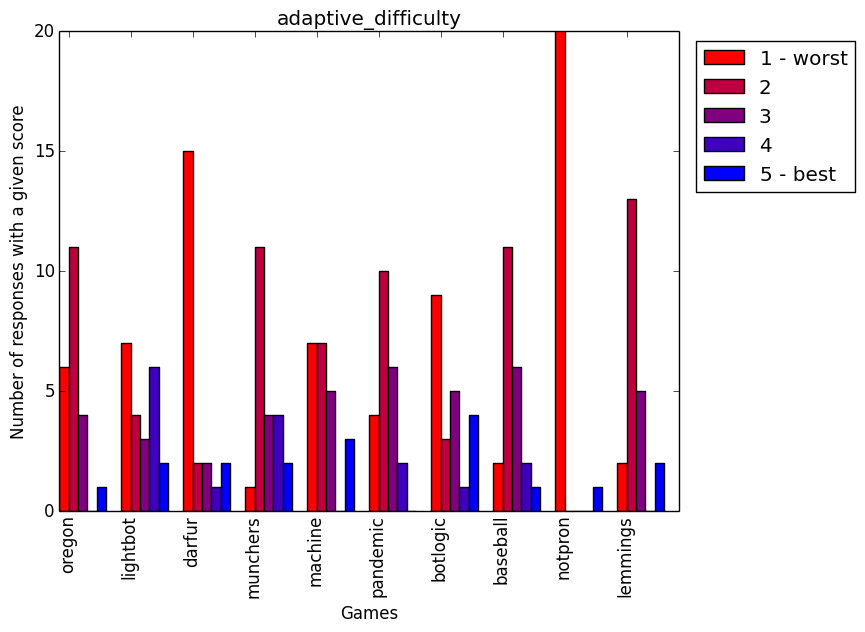
\includegraphics[height=0.33\textheight]{adaptive_difficulty_scores.png} 
			\caption{Adaptive Difficulty}
			\end{figure}

			\begin{figure}[h] 
			\centering 
			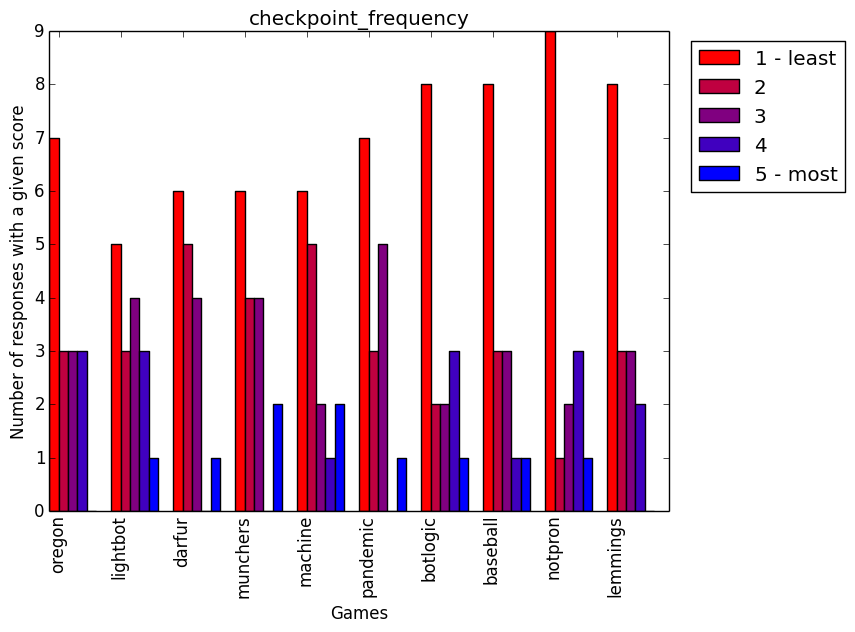
\includegraphics[height=0.33\textheight]{checkpoint_frequency_scores.png} 
			\caption{Checkpoint Frequency}
			\end{figure}

			\begin{figure}[h] 
			\centering 
			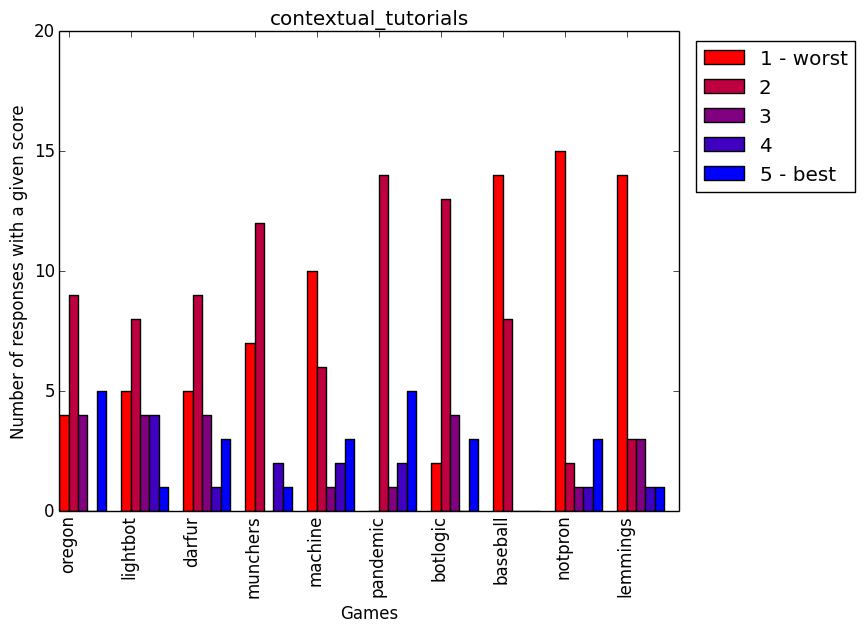
\includegraphics[height=0.33\textheight]{contextual_tutorials_scores.png} 
			\caption{Contextual Tutorials}
			\end{figure}

			\begin{figure}[h] 
			\centering 
			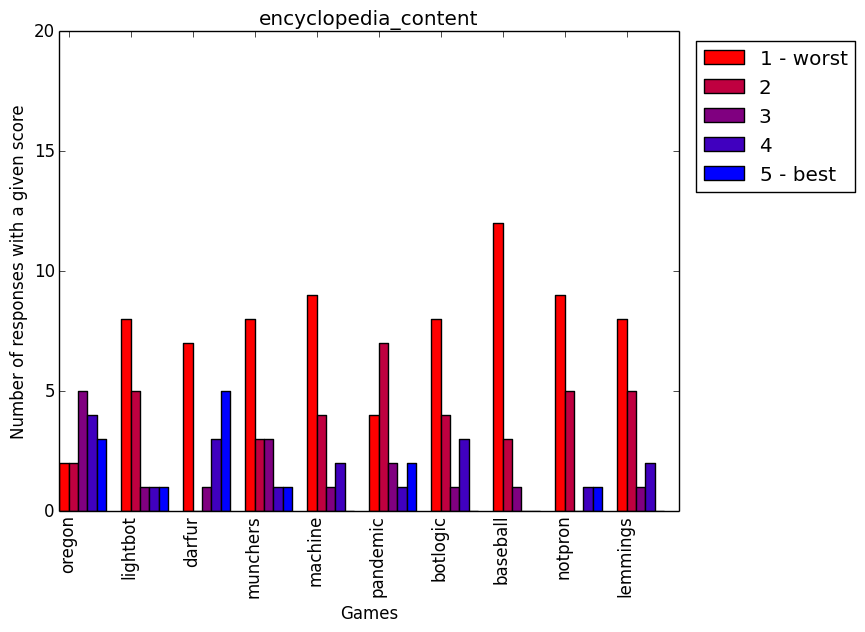
\includegraphics[height=0.33\textheight]{encyclopedia_content_scores.png} 
			\caption{Encyclopedia Content}
			\end{figure}

			\begin{figure}[h] 
			\centering 
			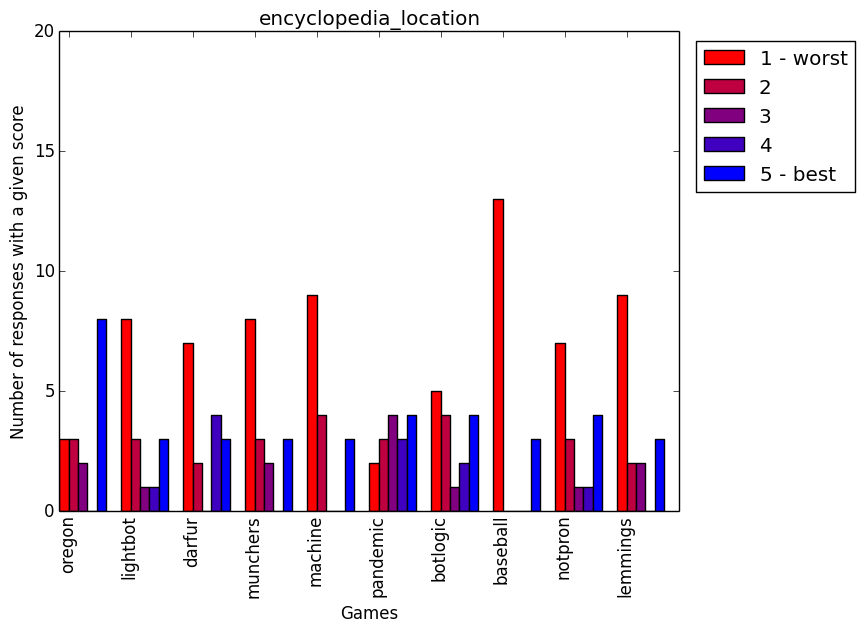
\includegraphics[height=0.33\textheight]{encyclopedia_location_scores.png} 
			\caption{Encyclopedia Location}
			\end{figure}

			\begin{figure}[h] 
			\centering 
			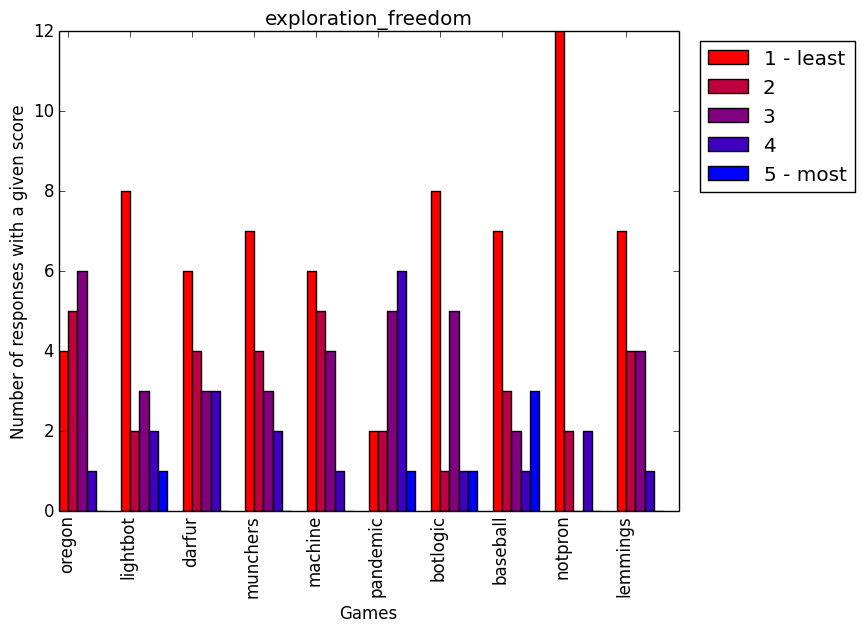
\includegraphics[height=0.33\textheight]{exploration_freedom_scores.png} 
			\caption{Freedom of exploration}
			\end{figure}

			\begin{figure}[h] 
			\centering 
			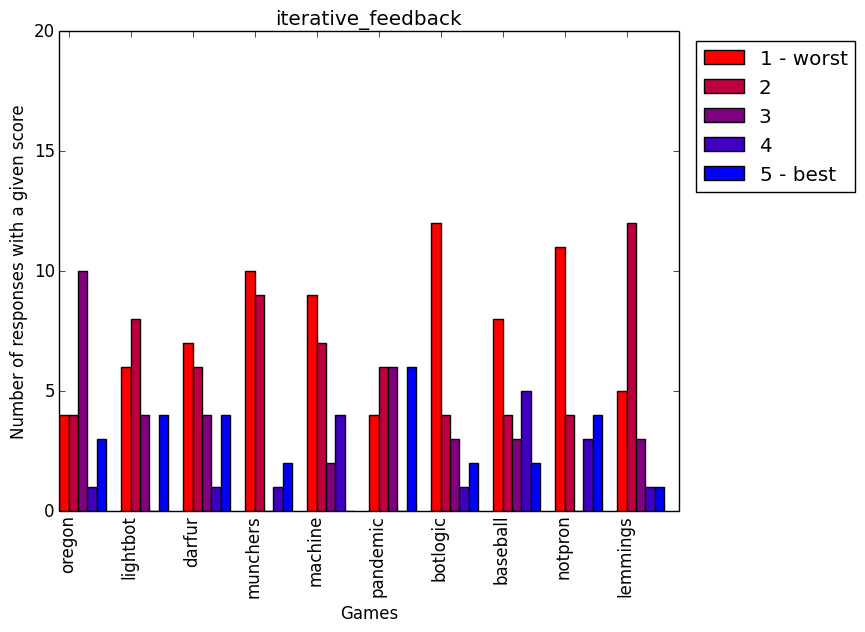
\includegraphics[height=0.33\textheight]{iterative_feedback_scores.png} 
			\caption{Iterative feedback}
			\end{figure}

			\begin{figure}[h] 
			\centering 
			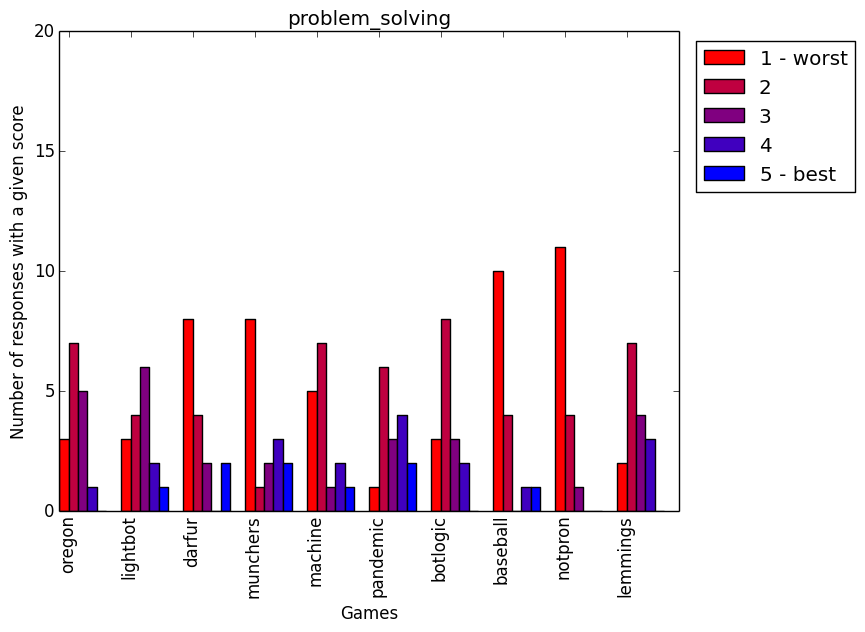
\includegraphics[height=0.33\textheight]{problem_solving_scores.png} 
			\caption{Unorthodox problem-solving}
			\end{figure}

			\begin{figure}[h] 
			\centering 
			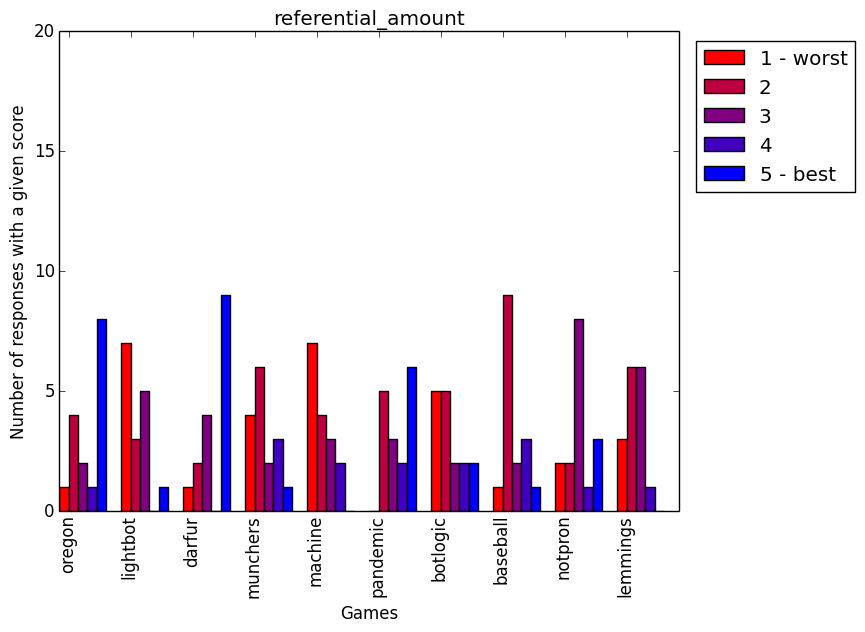
\includegraphics[height=0.33\textheight]{referential_amount_scores.png} 
			\caption{Amount of referential material}
			\end{figure}

			\begin{figure}[h] 
			\centering 
			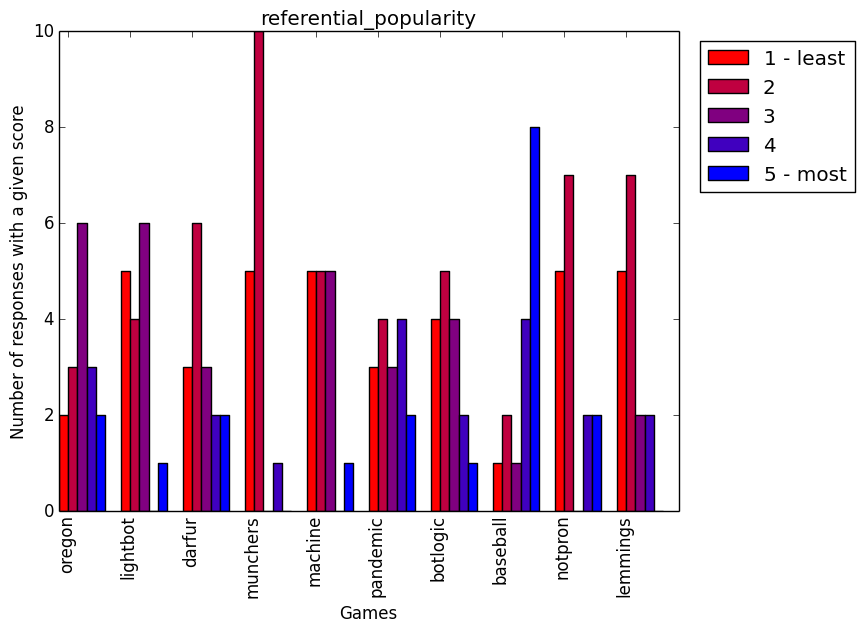
\includegraphics[height=0.33\textheight]{referential_popularity_scores.png} 
			\caption{Popularity of referential material}
			\end{figure}

			\begin{figure}[h] 
			\centering 
			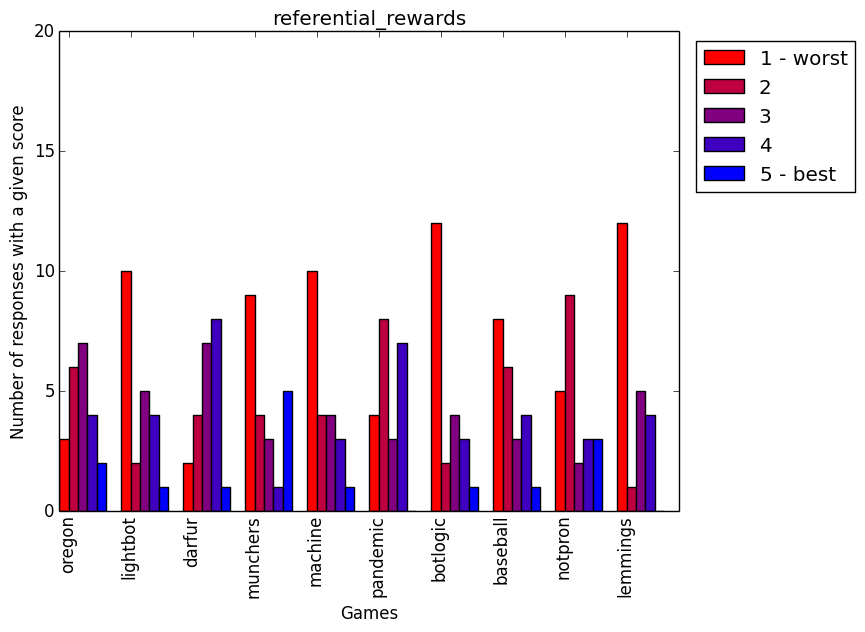
\includegraphics[height=0.33\textheight]{referential_rewards_scores.png} 
			\caption{Rewards for knowing referential material}
			\end{figure}

			\begin{figure}[h] 
			\centering 
			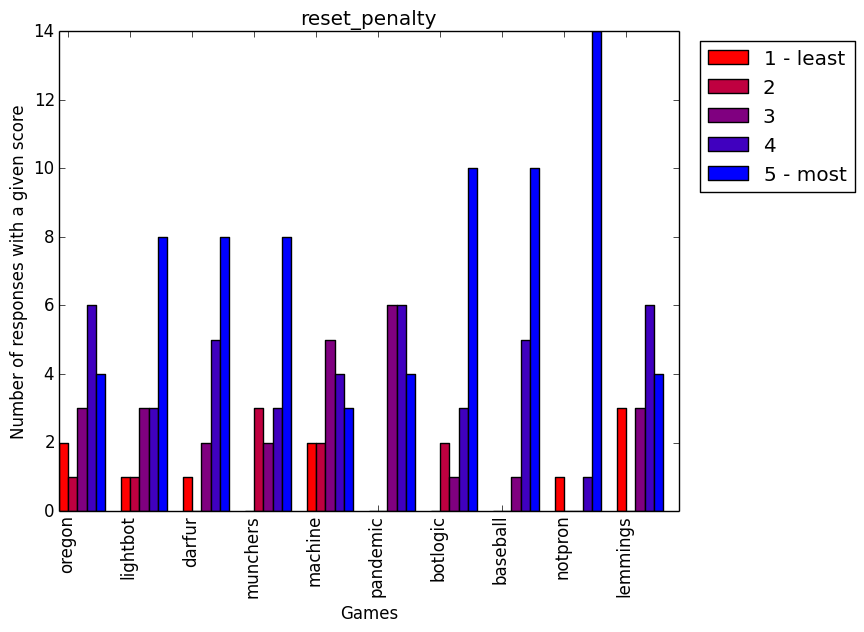
\includegraphics[height=0.33\textheight]{reset_penalty_scores.png} 
			\caption{Reset time penalty for failure}
			\end{figure}

			\begin{figure}[h] 
			\centering 
			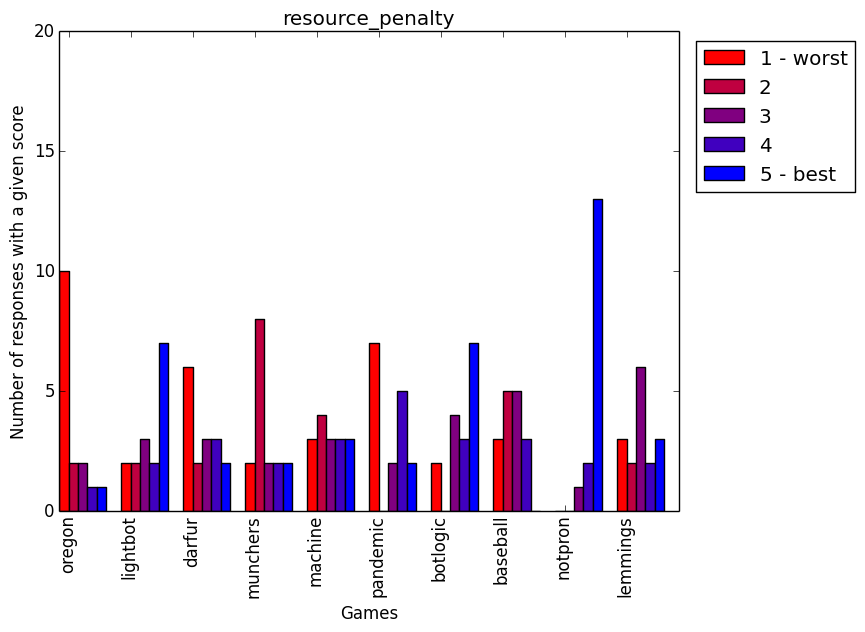
\includegraphics[height=0.33\textheight]{resource_penalty_scores.png} 
			\caption{Game resource penalty for failure}
			\end{figure}


\cleardoublepage
		\subsection{Game Scores}
			This section contains the scoring results for each game. For each game, a bar graph is given for each rubric item. The bar graph contains the scores that the rubric item recieved for that game.

			An alternate visualization of this data, where each rubric item has a bar graph for all of the game, can be found in the previous section.

			\begin{figure}[h] 
			\centering 
			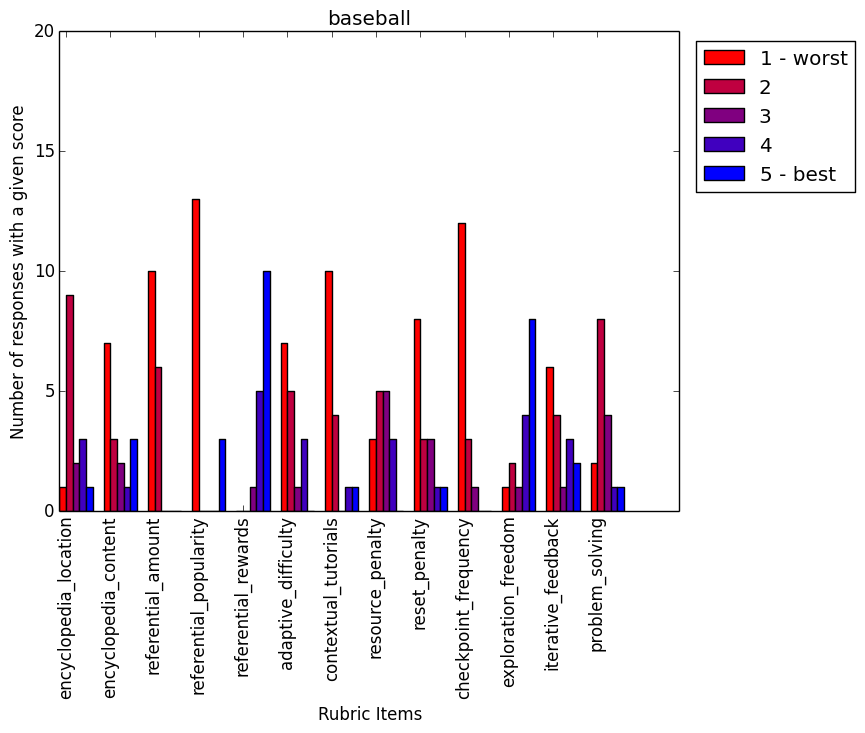
\includegraphics[height=0.33\textheight]{baseball_scores.png} 
			\caption{Math Baseball}
			\end{figure}

			\begin{figure}[h] 
			\centering 
			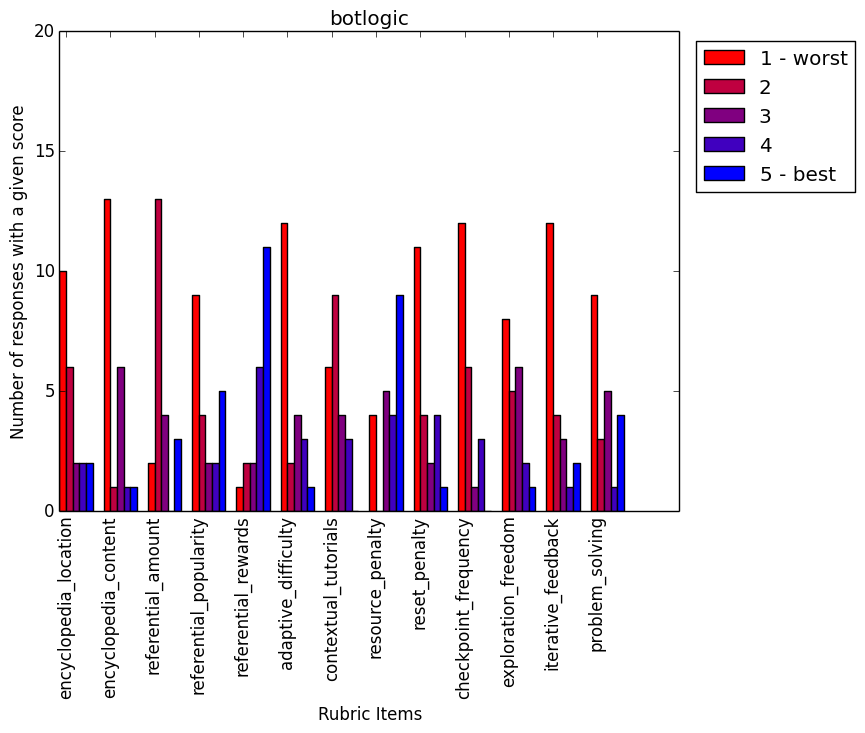
\includegraphics[height=0.33\textheight]{botlogic_scores.png} 
			\caption{Botlogic}
			\end{figure}

			\begin{figure}[h] 
			\centering 
			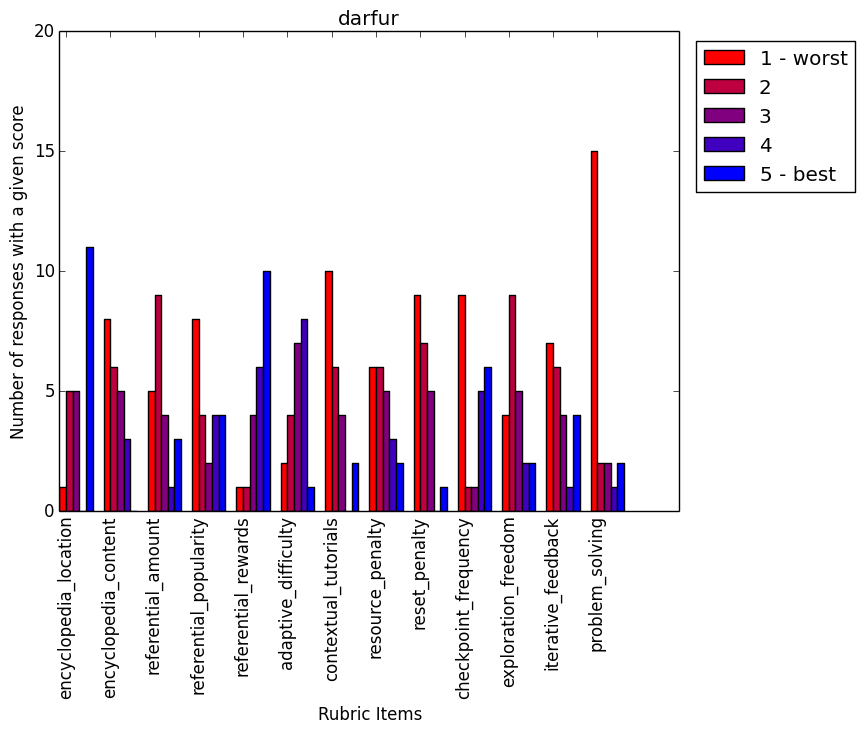
\includegraphics[height=0.33\textheight]{darfur_scores.png} 
			\caption{Darfur is Dying}
			\end{figure}

			\begin{figure}[h] 
			\centering 
			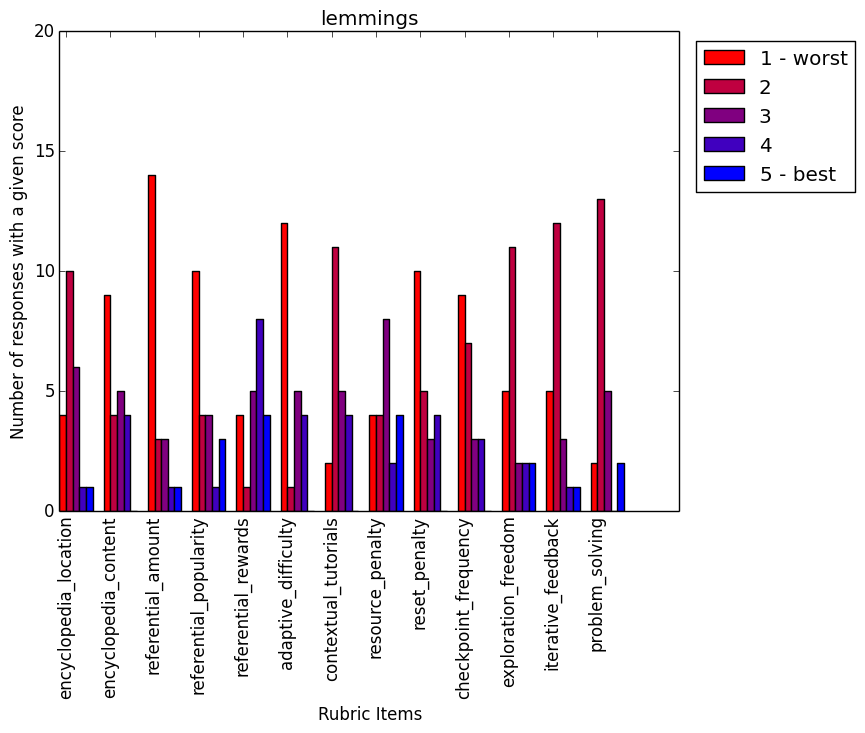
\includegraphics[height=0.33\textheight]{lemmings_scores.png} 
			\caption{Lemmings}
			\end{figure}

			\begin{figure}[h] 
			\centering 
			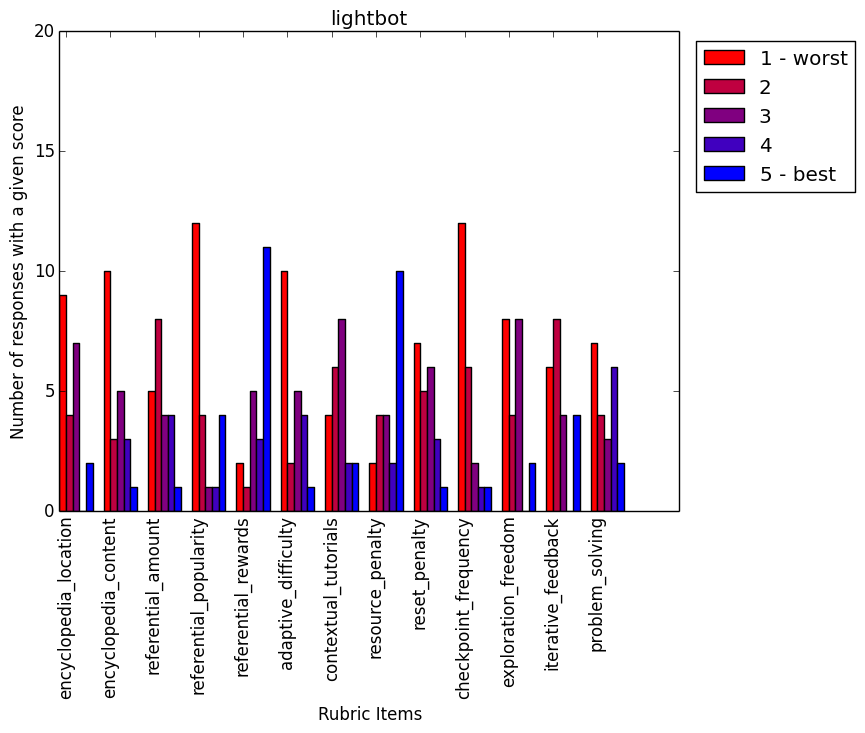
\includegraphics[height=0.33\textheight]{lightbot_scores.png} 
			\caption{Light Bot}
			\end{figure}

			\begin{figure}[h] 
			\centering 
			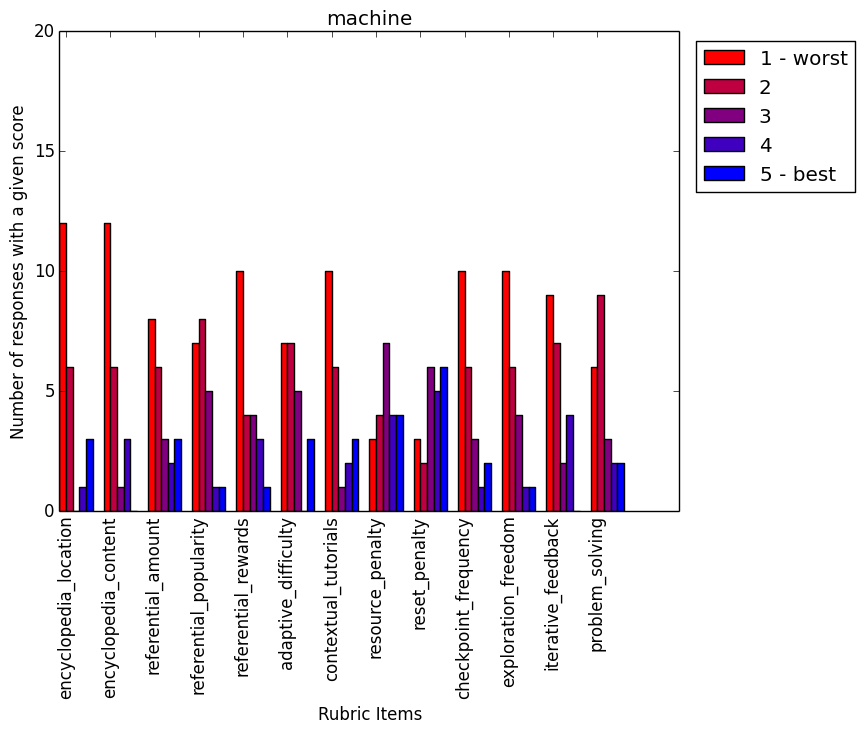
\includegraphics[height=0.33\textheight]{machine_scores.png} 
			\caption{The Incredible Machine}
			\end{figure}

			\begin{figure}[h] 
			\centering 
			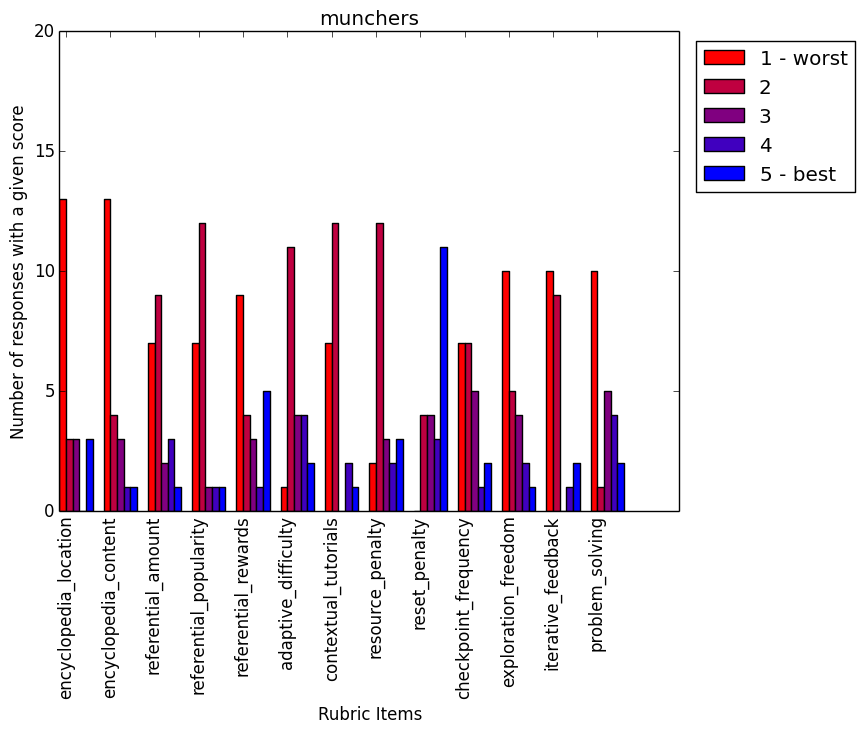
\includegraphics[height=0.33\textheight]{munchers_scores.png} 
			\caption{Number Munchers}
			\end{figure}

			\begin{figure}[h] 
			\centering 
			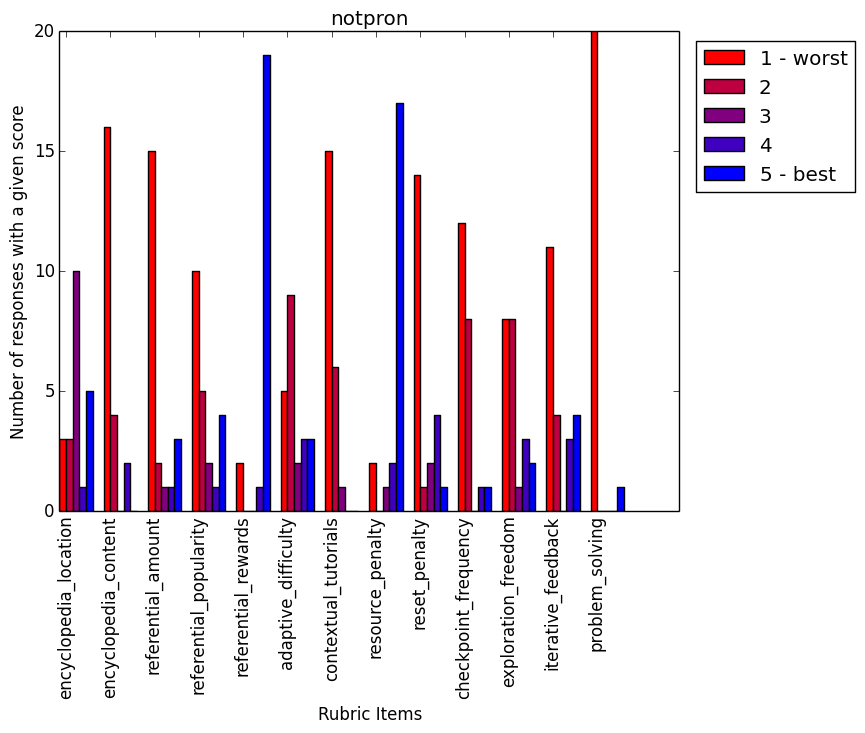
\includegraphics[height=0.33\textheight]{notpron_scores.png} 
			\caption{Notpron}
			\end{figure}


			\subsubsection{The Oregon Trail}
				\begin{figure}[h] 
				\centering 
				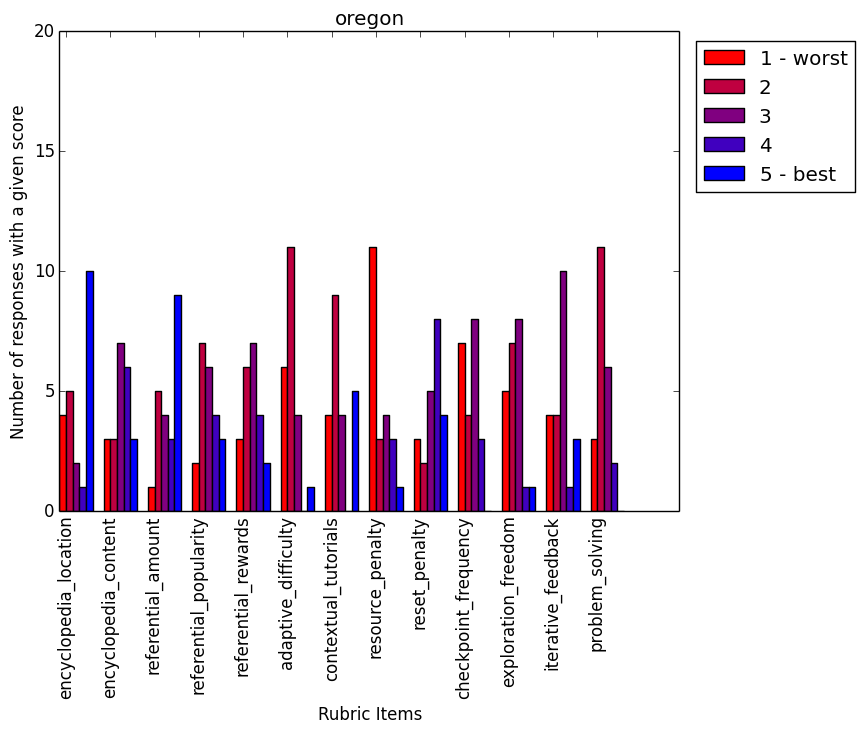
\includegraphics[height=0.33\textheight]{oregon_scores.png} 
				\caption{The Oregon Trail}
				\end{figure}

				It's important to note blah blah blah

			\begin{figure}[h] 
			\centering 
			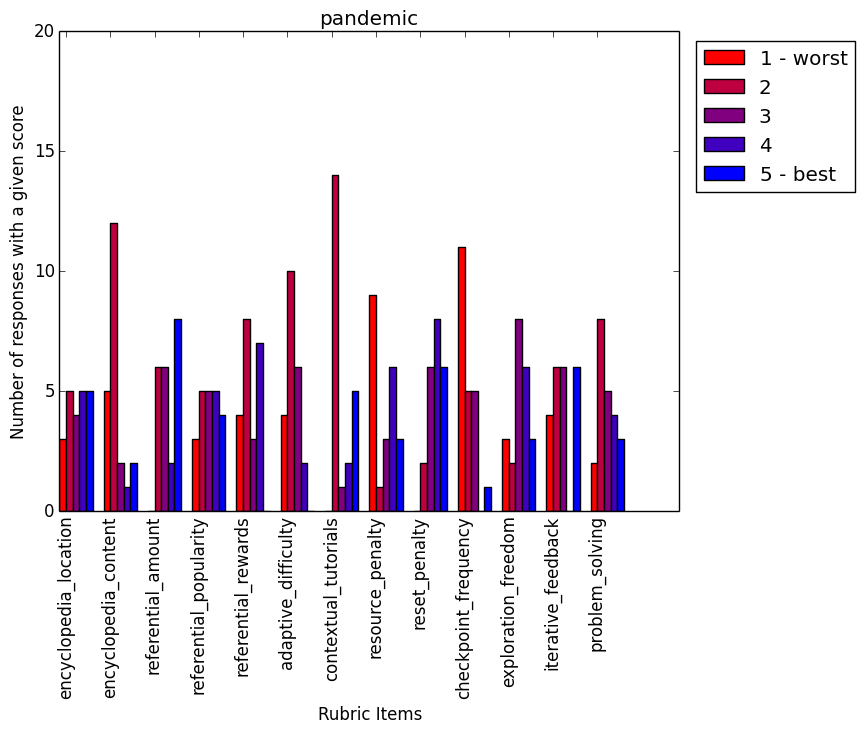
\includegraphics[height=0.33\textheight]{pandemic_scores.png} 
			\caption{Pandemic 2}
			\end{figure}

\cleardoublepage
